\documentclass{article}
\usepackage{geometry}
\usepackage{paralist}
\usepackage[T1]{fontenc}
\usepackage{reledmac}
\usepackage{changepage}
\usepackage{layout}

\usepackage{pgfplots}
\usepackage{tikz}
\usetikzlibrary{positioning}
\usetikzlibrary{shapes.geometric, arrows}
\usetikzlibrary{calc, shapes, backgrounds}
\tikzstyle{arrow} = [thick,->,>=stealth]

\usepackage{graphicx} 
\graphicspath{ {./images/} }

\usepackage{fancyhdr}
\fancyhead[L]{
	\begin{tabular}{l}
		\Large \textbf{\textsc{Distributed Systems}} \\
		\large Project 03 - Part 01
	\end{tabular}
}
\fancyhead[R]{
	\begin{tabular}{r}
		16-124-836 \\
		Marcel \textsc{Zauder}
	\end{tabular}
}
\renewcommand{\headrulewidth}{0.4pt}
\fancyfoot[C]{\thepage}
\renewcommand{\footrulewidth}{0.4pt}
\setlength{\headsep}{35pt}
\setlength{\textheight}{600pt}

\usepackage{hyperref}

\begin{document}
	\pagestyle{fancy}
	
	All required files are in their respective directories with specified names.	
	
	\section*{Task 02 - Redis Benchmark}
	\begin{adjustwidth}{2em}{2em}
		\begin{enumerate}[\tiny\textbullet]
			\item \textsc{Number of Requests}
			\begin{center}
				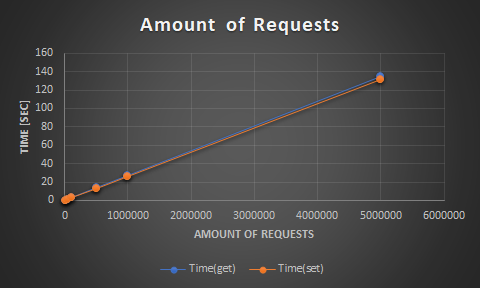
\includegraphics[scale=0.6]{Task_02_Requests.png}
			\end{center}
			\item \textsc{Data Size}
			\begin{adjustwidth}{-3em}{}
				\hfill \\
				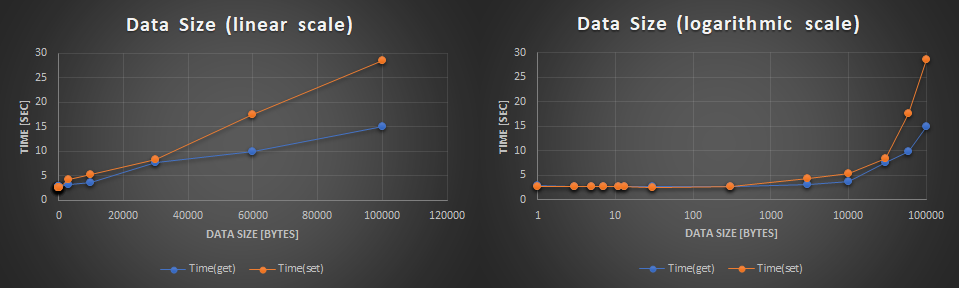
\includegraphics[scale=0.6]{Task_02_DataSize.png}
			\end{adjustwidth}
		\end{enumerate}
		\hfill \\
		When increasing the number of requests both times for the \textit{set} and \textit{get} commands are increasing linearly as well. Additionally there is no significant difference between those two times. \\
		As soon as the data size reaches 1000 Bytes the time increases in a linear way for both the \textit{set} and \textit{get} commands. Different to the amount of requests there is a significant difference between the both times of the commands. The \textit{set} command needs approximately twice the time for the same amount of commands than the \textit{get} command.
	\end{adjustwidth}
	
	\newpage
	
	\section*{Task 03 - Scale-Up Cluster}
	\begin{adjustwidth}{2em}{2em}
		\begin{enumerate}[\tiny\textbullet]
			\item \textsc{Number of Requests}
			\begin{center}
				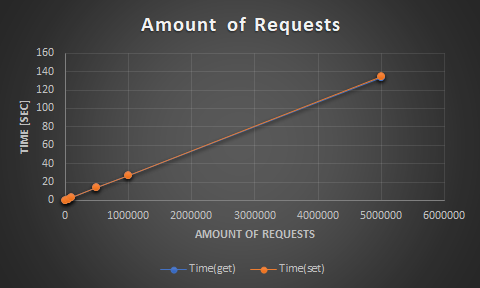
\includegraphics[scale=0.6]{Task_03_Requests.png}
			\end{center}
			\item \textsc{Data Size}
			\begin{adjustwidth}{-3em}{}
				\hfill \\
				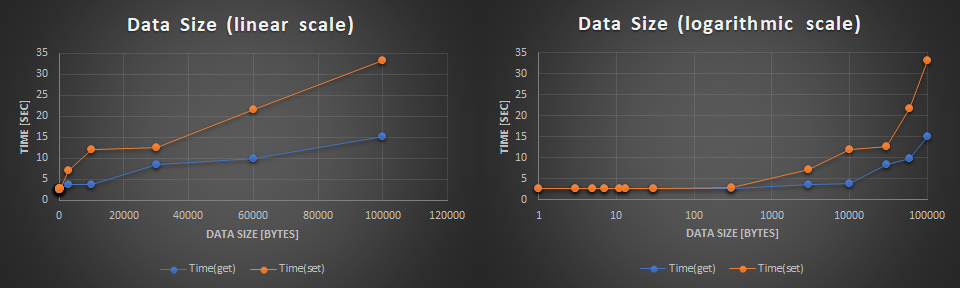
\includegraphics[scale=0.6]{Task_03_DataSize.png}
			\end{adjustwidth}
		\end{enumerate}
		\hfill \\
		As before the times are increasing linearly , but it must be pointed out that it takes up to 10\% more time for the same number of requests or the same data sizes then when only using one slave. Again the \textit{get} command needs less time than the \textit{set} command when increasing the data size.
	\end{adjustwidth}
	
	\newpage
	
	\section*{Task 04 - Full Benchmark}
	\begin{adjustwidth}{2em}{2em}
		\begin{enumerate}[\tiny\textbullet]
			\item \textsc{Number of Slaves}
			\begin{center}
				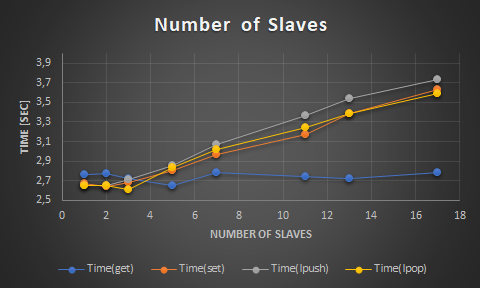
\includegraphics[scale=0.55]{Task_04_Slaves.png}
			\end{center}
			\item \textsc{Number of Sentinels}
			\begin{center}
				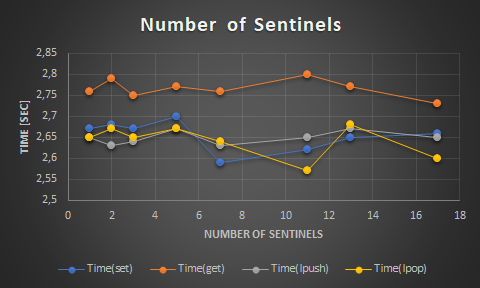
\includegraphics[scale=0.55]{Task_04_Sentinels.png}
			\end{center}
		\end{enumerate}
		\hfill \\
		When increasing the slave size the times for the \textit{set}, \textit{lpush}, and \textit{lpop} commands are steadily increasing. Only the time for the \textit{get} command stays constant. This implies that the master tries to execute a write command on every slave but only gets the information from one slave. Therefore it takes more time to get the acknowledge message from every slaves when writing a new information to them. \\
		Increasing the number of sentinels does not have a significant effect on the executing time.
	\end{adjustwidth}
	
	\section*{Task 05 - Sentinels}
	\begin{adjustwidth}{2em}{2em}
		We will take the log from sentinel 2 as an example: \\
		\hfill \\
		It gets interesting when the sentinel writes the following lines in the log:
		\begin{adjustwidth}{-4em}{-4em}
		\begin{center}
			\begin{tabular}{|l|}
			\hline
			\texttt{sentinel\_2  | 1:X 03 Dec 13:03:32.689 \# +sdown master mymaster 172.17.0.2 6379} \\
			\texttt{sentinel\_2  | 1:X 03 Dec 13:03:32.772 \# +odown master mymaster 172.17.0.2 6379 \#quorum 2/2} \\
			\texttt{sentinel\_2  | 1:X 03 Dec 13:03:32.772 \# +new-epoch 1} \\
			\hline
			\end{tabular}
		\end{center}
		\end{adjustwidth}
		\hfill \\
		In the first line the sentinel notices that his master is not available anymore and sends a message to all other sentinels that it has detected that the master is down/paused. In the next line it receives all the other messages that the master is down. such that the majority has detected this state and therefore a new epoch is started in line 3. \\
		At the start of the new epoch a new leader is elected by majority voting. In the end the master is switched to the address 172.17.0.6 6379. After that the sentinels are communicating with the new master as before when the old master was online.
	\end{adjustwidth}
\end{document}